% Generado por sistema/backend ReporteTex.java -- no editar a mano.
% Datos: CSV importado (titulados) / CSV importado (empleadores)
De los 148 titulados que respondieron, 25 declaran no estar trabajando actualmente (ni en una organización ni en un emprendimiento propio). La Tabla y el gráfico siguientes muestran la razón que indican, tomada como un factor de riesgo de desempleo.

\begin{mitabla}{Razón por la que actualmente no trabaja ($n=25$)}
\begin{tabular}{lccc}
\toprule
Razón & $f_i$ & $f_i / n$ & \% \\
\midrule
Demanda laboral inexistente & 6 & $6/25 = 0.240$ & 24.0 \\
Falta de experiencia previa & 4 & $4/25 = 0.160$ & 16.0 \\
Falta de habilidades específicas & 7 & $7/25 = 0.280$ & 28.0 \\
Red de contactos limitada & 1 & $1/25 = 0.040$ & 4.0 \\
Problemas con el CV & 0 & $0/25 = 0.000$ & 0.0 \\
Entrevistas & 1 & $1/25 = 0.040$ & 4.0 \\
Remuneración muy baja & 2 & $2/25 = 0.080$ & 8.0 \\
Otro & 4 & $4/25 = 0.160$ & 16.0 \\
\midrule
Total & 25 & & 100.0 \\
\bottomrule
\end{tabular}
\end{mitabla}

\textit{Lectura:} la respuesta más frecuente es ``Falta de habilidades específicas'' ($f_i = 7$, 28.0\% de 25).

\begin{figure}[H]
\centering
\caption{Razón por la que actualmente no trabaja ($n=25$)}
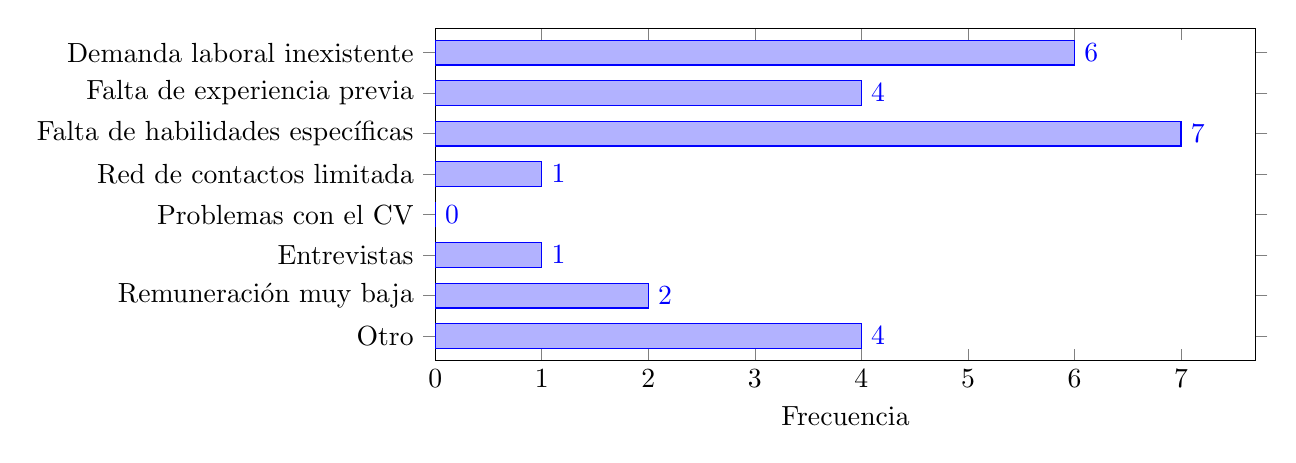
\begin{tikzpicture}
\begin{axis}[
  xbar, bar width=9pt,
  width=12cm, height=5.8cm,
  xlabel={Frecuencia}, xmin=0,
  ytick={0,...,7},
  yticklabels={Demanda laboral inexistente,Falta de experiencia previa,Falta de habilidades específicas,Red de contactos limitada,Problemas con el CV,Entrevistas,Remuneración muy baja,Otro},
  ymin=-0.6, ymax=7.6,
  nodes near coords, y dir=reverse,
  every axis plot/.style={fill=gray!60}
]
\addplot coordinates {(6,0) (4,1) (7,2) (1,3) (0,4) (1,5) (2,6) (4,7) };
\end{axis}
\end{tikzpicture}
\end{figure}

Esta razón declarada no es el único factor de riesgo que registra el estudio: los cruces C12 (edad $\times$ situación laboral) y C14 (formación complementaria $\times$ situación laboral) de la Sección~\ref{sec:cruces} prueban estadísticamente si la edad y la formación complementaria también se asocian con el riesgo de no tener trabajo.

